\section{Rappel des règles du jeu}

Il s’agit d’un jeu tour-par-tour inspiré de \og Small World \fg{}, dans lequel chaque joueur dirige un peuple. Le but du jeu est de gérer des unités sur une carte pour obtenir le plus de points possible, à la fin d’un certain nombre de tours. Pour ce faire, chaque joueur commence avec toutes ses unités placées sur une même case de la carte. Il doit ensuite les répartir au mieux sur les différentes cases de la carte : par défaut, une case rapporte 1 point (hors bonus/malus). Les unités d’un joueur peuvent également attaquer les unités de l'autre pour les détruire (limitant ainsi l’acquisition de points de l’adversaire) et occuper une case de la carte. 

\subsection{Les peuples et leurs unités}

Il existe trois peuples \textit{Elf}, \textit{Orc}, et \textit{Nain}, ayant des caractéristiques très différentes :

\begin{itemize}

\item \textbf{Elf} :  le coût de déplacement sur une case Forêt est divisé par deux. Le coût de déplacement sur une case Désert est multiplié par deux.
\item \textbf{Orc} : le coût de déplacement sur une case Plaine est divisé par deux. Une unité Orc n’acquière aucun point sur les cases de type Forêt. Lorsqu’une unité Orc détruit une autre unité, elle possède alors 1 point de bonus permanent. Cet effet est cumulable et est lié à chaque unité (i.e. si l’unité ayant le bonus meurt, le bonus disparaît).
\item \textbf{Nain} :  le coût de déplacement sur une case Plaine est divisé par deux. Une unité Nain n’acquière aucun point sur les cases Plaine. Lorsqu’elle se trouve sur une case Montagne, une unité Nain peut se déplacer sur n’importe quelle case Montagne de la carte, à condition qu’elle ne soit pas occupée par une unité adverse.

\end{itemize}

Lors d'un tour, toutes les unités du peuple peuvent être déplacées et attaquer. Par défaut, chaque unité possède 2 points de mouvement, et chaque déplacement en coûte un (hors bonus/malus). Cela signifie qu’une même unité peut se déplacer plusieurs fois par tour. Chaque unité possède en plus à la base 2 points d’attaque, 1 point de défense et 5 points de vie. Les unités ne récupèrent pas leurs points de vie à la fin d’un tour, mais leurs points de déplacement sont réinitialisés à 2 à chaque tour.

\subsection{Le plateau de jeu}

La carte du monde se compose de quatre types de cases (hexagonales) : \textit{Plaine}, \textit{Désert}, \textit{Montagne} , \textit{Forêt}.

Il existe 3 tailles de carte, auxquelles sont associées un nombre de tours ainsi qu'un nombre d'unités :

\begin{itemize}

\item \textbf{Petite} (\textit{Small}) : 6 * 6 cases, 5 tours, 4 unités par peuple.
\item \textbf{Moyenne} (\textit{Medium}) : 10 * 10 cases, 20 tours, 6 unités par peuple.
\item \textbf{Grande} (\textit{Large}) : 14 * 14 cases, 30 tours, 8 unités par peuple.

\end{itemize}

La carte, ainsi que les unités des deux peuples, sont visibles par les deux joueurs. La carte est vue du dessus.

\section{Guide d'utilisation}

\subsection{Lancement du jeu}

Pour lancer le jeu, 

\begin{figure}[!h]
    \centering
    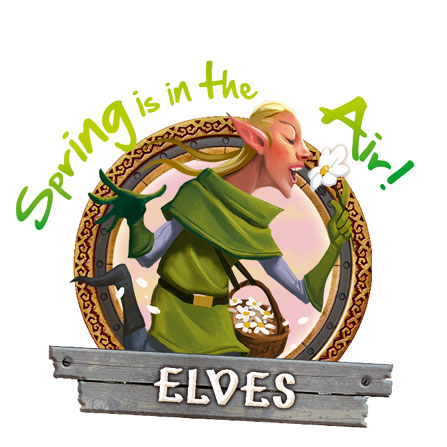
\includegraphics[height=0.70\textwidth]{figure/ecranAccueil.png}
    \caption{Page d'accueil du jeu.}
    \label{fig:ecranAccueil}
\end{figure} 

C'est à partir de cet écran d'accueil que vous allez pouvoir créer une nouvelle partie.

\subsection{Créer une partie}

Pour créer une nouvelle partie à partir de l'écran d'accueil, cliquez sur \og Create new game \fg{}. Une boîte de dialogue s'affiche alors, par laquelle il faut choisir la taille de la carte par sélection dans la liste déroulante dont vous avez un aperçu à la {\sc Figure}~\ref{fig:sizeMap}. Après validation, une nouvelle fenêtre s'affiche et chaque joueur doit choisir son peuple (une vérification a été mise en place afin de s'assurer que les peuples choisis soient différents). Cette fenêtre est similaire à celle de la {\sc Figure}~\ref{fig:choicePeoples}. Après cette dernière étape, vous pouvez alors commencer la partie en cliquant sur \og Valider \fg{}.

\begin{figure}[!h]
    \centering
    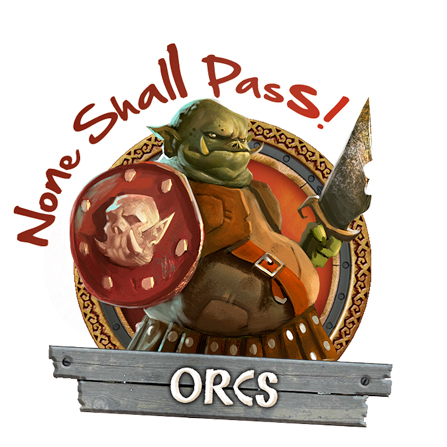
\includegraphics[height=0.60\textwidth]{figure/sizeMap.png}
    \caption{Choix de la taille de la carte.}
    \label{fig:sizeMap}
\end{figure}

\begin{figure}[!h]
    \centering
    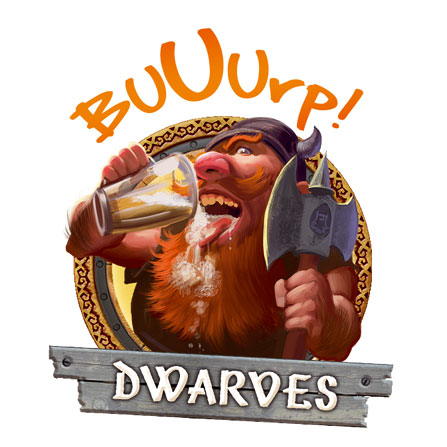
\includegraphics[height=0.60\textwidth]{figure/choicePeoples.png}
    \caption{Choix des peuples des joueurs 1 et 2.}
    \label{fig:choicePeoples}
\end{figure}

\begin{landscape}
    \begin{figure}[!h]
    \centering
    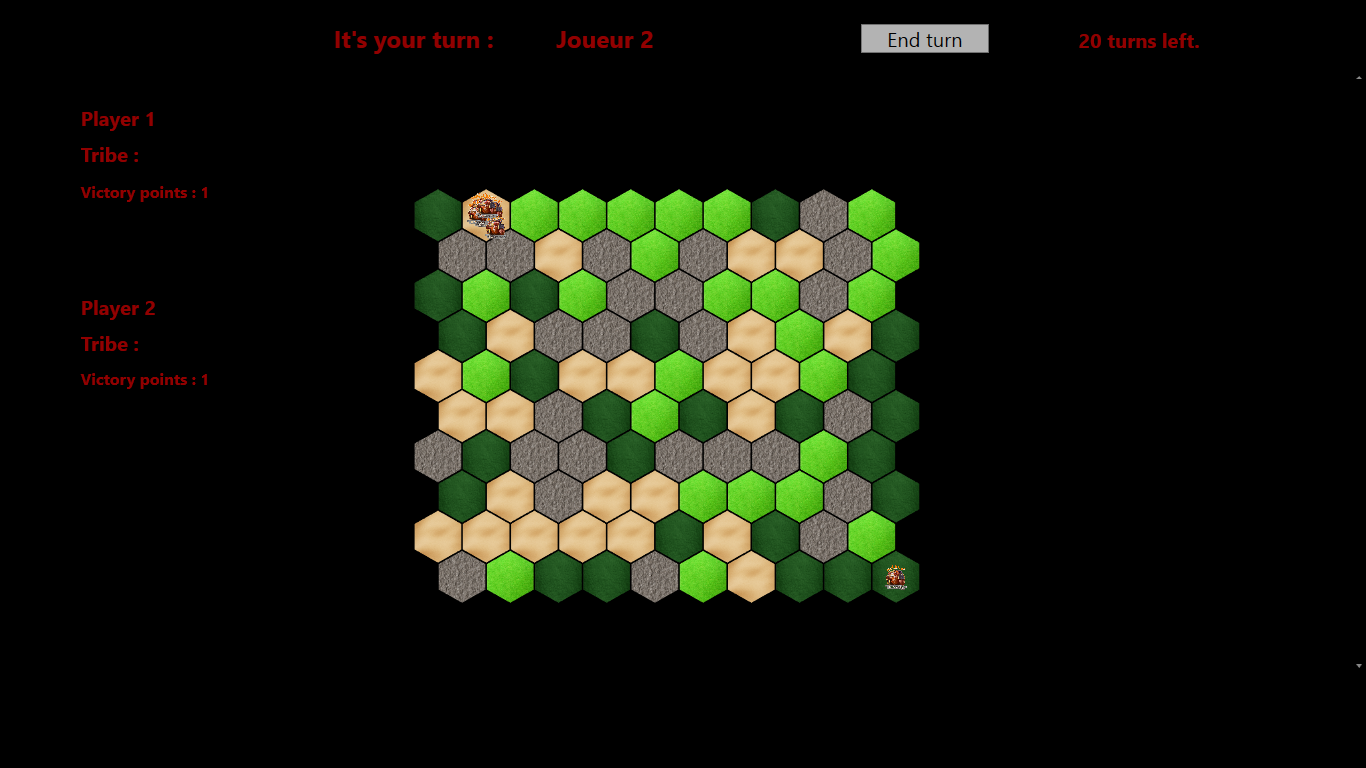
\includegraphics[height=0.90\textwidth]{figure/game.png}
    \caption{Interface globale du jeu.}
    \label{fig:game}
    \end{figure}
\end{landscape}

\subsection{Interface du jeu}

La {\sc Figure}~\ref{fig:game} montre un aperçu de l'interface globale du jeu (avec une carte de taille Medium). Différents éléments sont accessibles et/ou manipulables à partir de cette dernière.

\subsubsection{Les données des joueurs}

Vous pouvez voir, à gauche de la carte, le nombre de points de chacun des joueurs (recalculé à chaque nouveau tour). À droite de la carte est également affichée la liste des unités sélectionnées. 

\subsubsection{La carte}

Au début du jeu, toutes les unités de chaque peuple (et donc d'un même joueur) sont regroupées sur une même case. Les deux peuples sont initialement positionnés de façon à être le plus loin possible l'un de l'autre. Le premier joueur (désigné aléatoirement) peut alors commencer à déplacer ses unités. La case sur laquelle se trouve le curseur de la souris est entourée de blanc, comme sur la {\sc Figure}~\ref{fig:sizeMap}, et s'assombrit lorsque le joueur la sélectionne.

\begin{figure}[!h]
    \centering
    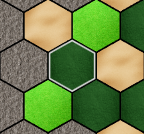
\includegraphics[height=0.40\textwidth]{figure/selectSpace.png}
    \caption{Au milieu : passage de la souris au-dessus d'une case.}
    \label{fig:onSpace}
\end{figure}

\subsubsection{Le déplacement des unités}

Les unités peuvent seulement se déplacer sur les cases ayant un côté en commun avec la leur (excepté les Nains qui ont un accès spécial aux cases \textit{Montagne}). Pour faire bouger l'unité courante, il vous suffit de cliquer sur la case voulue. Si le déplacement est conforme aux règles du jeu, l'unité est repositionnée. Sinon, rien ne se passe et vous pouvez réessayer jusqu'à trouver une case qui fonctionne. Un autre mouvement sera ensuite possible si l'unité dispose encore de suffisamment de points de déplacement.

\subsubsection{Les combats}

Un combat a lieu automatiquement lorsqu'une unité a été déplacée sur une case comportant une unité adverse (ou plusieurs, auquel cas l'unité défensive la plus forte sera désignée pour se battre). Quel que soit le gagnant du combat, l'attaquant perd le même nombre de points de mouvements que lors d'un déplacement normal. Cependant, si la bataille mène à la mort de l'unité attaquée et que sa case est alors vide, l'unité attaquante est déplacée dessus.

\subsubsection{Fin du tour}

À n'importe quel moment du tour, même si vous n'avez pas déplacé toutes vos unités, il est possible de passer au tour suivant en cliquant sur le bouton \og End turn \fg{} en haut à droite de l'interface (voir {\sc Figure}~\ref{fig:game}). S'il reste encore au moins un tour, le joueur suivant pourra alors jouer, dans le cas contraire le jeu prendra fin.

\subsubsection{Fin du jeu}

Le jeu se termine de façon automatique si le nombre de tours fixé lors de la création de la partie a été atteint, ou si l'un des joueurs n'a plus aucune unité vivante. Le vainqueur est alors le joueur ayant le nombre de points le plus élevé. Cependant, il est possible de quitter le jeu à tout moment en appuyant sur la touche \og Echap \fg{}, puis en cliquant sur le bouton \og Quit game \fg{} visible sur la {\sc Figure}~\ref{fig:echap}. À partir ce menu, vous pouvez aussi revenir à la partie en cliquant sur \og Continue game \fg{}.

\begin{figure}
    \centering
    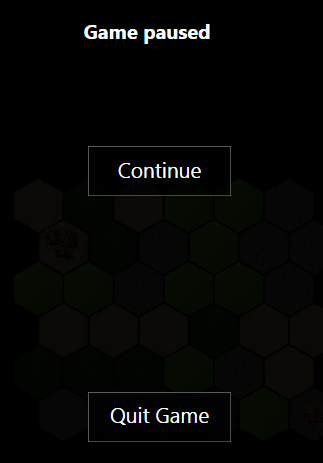
\includegraphics[height=0.60\textwidth]{figure/echap.png}
    \caption{Menu obtenu par pression de la touche Echap.}
    \label{fig:echap}
\end{figure}